\section{Formulating the conjecture}

From now on we will focus on $2$-coupon colorings and planar graphs.
A conjecture of Goddard and Henning \cite{gh} is the following.

\begin{conj}
  If $G$ is a simple triangulated planar graph of order at least $4$, then the
  total domatic number of $G$ is at least $2$.
\end{conj}

\begin{remark}
  The simplicity of the graph is necessary. Suppose the graph on figure
  \ref{fig:parallel} has a $2$-coupon coloring. Then $A$ and $C$ must have
  different colors, because they are the only neighbors of $B$. Similarly, $C$
  and $E$ must have different colors, as well as $E$ and $A$. That is a
  contradiction, since $A$, $C$ and $E$ form a triangle.
\end{remark}

\begin{figure}[h]
  \centering
  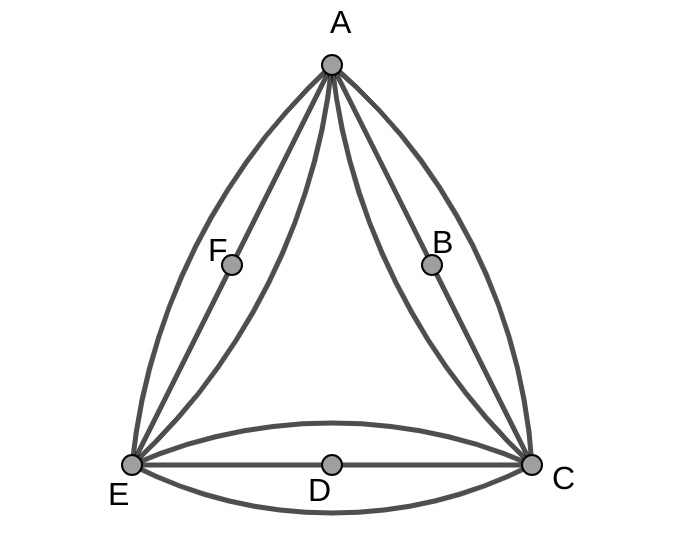
\includegraphics[width=70mm]{parallel}
  \caption{Simplicity is necessary}
  \label{fig:parallel}
\end{figure}

\begin{remark}
  Allowing triangulated disks (i.e. planar graphs with at most one face greater
  than $3$), the conjecture does not hold. For example, the graph on figure
  \ref{fig:sungraph} does not have a $2$-coupon coloring for similar reasons as
  the previous one. We will show later that this graph is a member of a bigger
  graph family without $2$ disjoint dominating sets.
\end{remark}

\begin{figure}[ht]
  \centering
  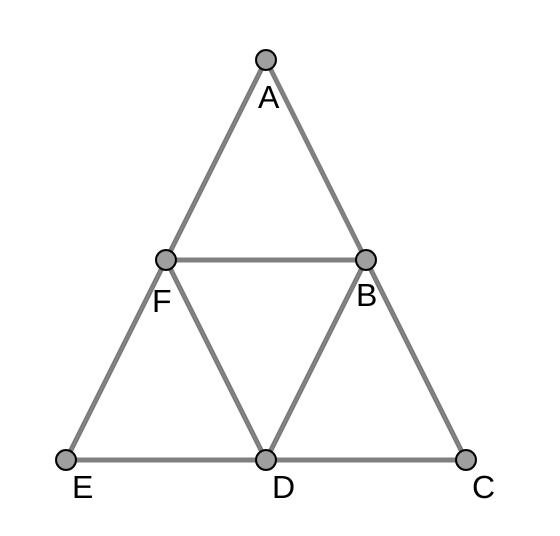
\includegraphics[width=70mm]{sungraph}
  \caption{The conjecture does not hold for triangulated disks}
  \label{fig:sungraph}
\end{figure}

\section{Easy proofs for some special cases}

There are some sufficient conditions known for having a total domatic number of
at least $2$. We will cover most of the known cases along the way. In this section
we take a look at special cases with relatively easy proofs.

The first example is a graph family for which an easy induction shows that they
are $2$-coupon colorable.

\begin{definition}
  A graph is called a stacked graph if it can be constructed from a triangle by
  repeatedly putting a new vertex in a face and connecting it with the vertices on
  the boundary of that face.
\end{definition}
\begin{remark}
  Stacked graphs are triangulated.
\end{remark}
\begin{claim}
  Stacked graphs with at least $4$ vertices are $2$-coupon colorable.
\end{claim}
\begin{proof}
  We can determine the colors of the vertices as the graph is constructed. The
  current coloring will maintain two following two properties.
  \begin{enumerate}
    \item It is a $2$-coupon coloring of the current graph.
    \item Every face has vertices from both color classes.
  \end{enumerate}
  The construction of the graph starts with a simple triangle. Color two vertices
  of the triangle to black, and the remaining vertex to white. Color the vertex added
  to the graph in the first step to white. This coloring has the desired properties.
  When a vertex is inserted into a face, color the new vertex to white if there is
  only one white vertex on the face's boundary, and black otherwise. This trivially
  maintains the desired properties.
\end{proof}

Goddard and Henning \cite{gh} verified the conjecture for several cases. We show now three
of them.

\begin{claim} \label{c:odd}
  Let $G$ be a simple triangulated graph. If all the
  vertices of $G$ have an odd degree, then there exists a coupon coloring with $2$ colors.
\end{claim}
\begin{proof}
  There exists a proper $4$-coloring of the vertices. As every vertex $v$ has an
  odd degree, there exists an odd cycle in the neighborhood of $v$. Hence, in a proper
  $4$-coloring $v$ has neighbors from at least $3$ color classes. This means that
  the union of any two color classes forms a total dominating set.
\end{proof}

\begin{claim}
  If $G$ can be obtained from a triangulated graph $H$ by putting a new vertex on every
  face and connecting them with the vertices of that face, then $G$ is $2$-coupon
  colorable.
\end{claim}
\begin{proof}
  Take a proper $4$-coloring on the vertices of $H$ and define a $2$-coloring by taking
  the union of $2-2$ color classes. The obtained coloring has the property that
  none of the faces is monochromatic. Color the additional vertices to black if the face
  has only one black vertex, and color it to white otherwise.
\end{proof}

\begin{claim} \label{ham_dual}
  Let $G$ be a a simple triangulated graph of order at least $4$. If the dual
  of $G$ is Hamiltonian, then $G$ admits two disjoint total dominating sets.
\end{claim}
\begin{proof}
  Let $C$ be the Hamiltonian cycle in the dual graph $G^*$. Consider $C$ as a curve on the plane.
  Color the vertices of $G$ inside $C$ to black, and the vertices outside of $C$ to white.
  We claim that this way we defined a $2$-coupon coloring of $G$. To prove this, we need to show
  that for every face $f$ of $G^*$, there exist a face $f'$ inside $C$ and a face $f''$
  outside of $C$ (inclusively) such that $f$ has a common edge with both $f'$ and $f''$.

  Let $f$ be a face inside $C$. We claim that $f$ has an edge on $C$. Otherwise the
  vertices of $f$ would be of degree at least $4$, which is a contradiction, as $G^*$ is
  $3$-regular. Let $f''$ be the face on the other side of this edge.

  If $f$ has a neighboring face inside $C$, then choose $f'$ to be that face.
  If $f$ does not have any neighboring faces inside $C$, then $f$ must be a face defined by $C$.
  As $G$ does not have parallel edges, all the edges of $C$ must belong to different
  faces outside of $C$. Index the vertices along $C$ from $c_1$ to $c_{n^*}$. If there
  is an edge $c_ic_j$ going between two non-consecutive vertices of $C$, then by the $3$-regularity
  of $G^*$, $c_ic_{i+1}$ and $c_{j - 1}c_j$ belong to the same face outside of $C$. It
  also follows from the $3$-regularity, that if there are two parallel $c_ic_{i+1}$ edges in $G^*$, then
  there is only one $c_{i + 1}c_{i + 2}$ edge. Thus, the only case in which all the edges of $C$
  belong to different faces outside of $C$, is when $C$ is of length $2$. This means, that
  $G$ is a triangle, and that is a contradiction.

  The same proof works for faces outside of $C$.
\end{proof}

\section{Variations of the conjecture}

As a reminder: the Goddard-Henning conjecture states that every simple triangulated
planar graph of order at least $4$ has total domatic number at least $2$. In this
chapter we try to find equivalent statements to the
conjecture, as well as (hopefully) slightly stronger statements. The motivation for
this chapter is that even if the stronger
statements are not true, they can be useful for proving the conjecture in special cases.

\begin{definition}
  Let $G$ be a triangulated planar graph. For a vertex $v$, each triangle
  containing $v$ has an edge not containing $v$. We call the cycle consisting of
  these edges a wheel.
\end{definition}

\begin{figure}[ht]
  \centering
  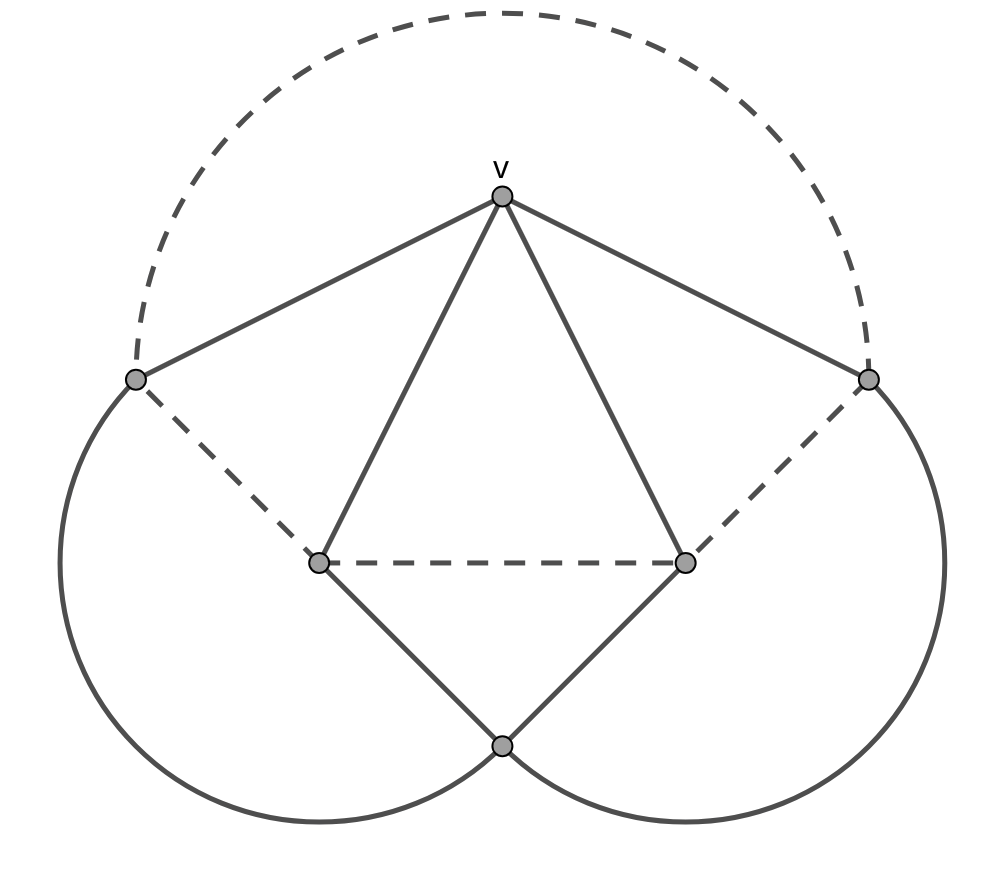
\includegraphics[width=70mm]{wheel}
  \caption{The green edges form the wheel defined by $A$ }
  \label{fig:wheel}
\end{figure}

\begin{guess}\label{s:bipartite}
  Let $G = (V, E)$ be a simple triangulated graph of order at least $4$. Then there
  exists a bipartite $H = (V, F)$ subgraph of $G$ such that $F$ contains at
  least one edge from each wheel of $G$.
\end{guess}

\begin{claim}
  The Goddard-Henning conjecture holds if and only if Statement \ref{s:bipartite} holds.
\end{claim}
\begin{proof}
  Let $G$ be a triangulated graph. Suppose first that it has a $2$-coupon coloring.
  $$F = \{uv \in E\ |\ u\ \textrm{and}\ v\ \textrm{are in different color classes}\}$$
  defines a bipartite subgraph of $G$ that contains at least one edge from each wheel.

  Now suppose that there exists bipartite subgraph that meets our requirement. Color
  the vertices in one of the classes to black, and the vertices in the other class
  to white. This is a $2$-coupon coloring of the original graph.
\end{proof}

\begin{guess}\label{s:forest}
  Let $G = (V, E)$ be a simple triangulated graph of order at least $4$. Then there
  exists a forest in $G$ containing at least one edge from each wheel.
\end{guess}

\begin{remark}
  If Statement \ref{s:forest} holds, then Statement \ref{s:bipartite} also holds.
\end{remark}

\begin{guess}\label{s:no_iso}
  Let $G = (V, E)$ be a simple triangulated graph of order at least $4$. Then there
  exists a subgraph $H' = (V, F')$ having the following two properties.
  \begin{enumerate}
    \item $F'$ contains exactly $1$ edge from each face of $G$.
    \item There are no isolated vertices in $H'$.
  \end{enumerate}
\end{guess}

\begin{lemma}\label{l:bipartite}
  A connected planar graph is bipartite if and only if each of its faces have an
  even number of edges.
\end{lemma}
\begin{proof}
  Suppose that the graph is not bipartite and thus there exists a cycle $C$ of odd
  length. We show that there exists an odd face. The proof goes by induction on the
  number of faces in the inner side of $C$. If $C$ is a face, then we are done.
  If $C$ is not a face, then there exists a face $f$ in the inner side of $C$ having at least one
  common edge with $C$. $f$ does not contain every edge of $C$, since $G$ is connected.
  Let $C'$ be the symmetric difference of the edge sets of $C$ and $f$. By the parity of $C$
  either $f$ is an odd face or $C'$ is an odd cycle containing less faces in its
  inner side than $C$.

  The other direction is trivial.
\end{proof}

\begin{claim}
  Statement \ref{s:no_iso} holds if and only if Statement \ref{s:bipartite} (and thus
  the Goddard-Henning conjecture) also holds.
\end{claim}
\begin{proof}
  Let $H' = (V, F')$ be the subgraph required by Statement \ref{s:no_iso}.
  We show that $H = (V, E - F')$ is a subgraph required by Statement \ref{s:bipartite}.
  $H$ is a bipartite graph by Lemma \ref{l:bipartite}, as each of its faces have $4$ edges.
  Take a wheel $v_1v_2\dots v_k$ defined by a vertex $v$. $v$ is not an isolated vertex in $H'$, so
  there exists a vertex $v_i$ such that $vv_i \in F'$. As $F'$ contains exactly one edge
  from each face, $v_iv_{i + 1} \in F$.

  \vspace{0.4cm}

  Now let $H = (V, F)$ be the subgraph required by Statement \ref{s:bipartite}.
  Clearly, $F$ cannot contain all three edges of a face.
  We show that there exists an edge set $F_0$, such that $(V, F \cup F_0)$ is a bipartite
  subgraph of $G$ that contains exactly two edges of each face. Let $F_0 = \emptyset$.
  We will add edges to $F_0$ maintaining that $(V, F \cup F_0)$ is a bipartite graph.

  Suppose that there exists a face $uvw$ in $G$ with $uv, vw \notin F \cup F_0$, $wu \in F \cup F_0$.
  If $F \cup F_0 \cup \{ uv \}$ or $F \cup F_0 \cup \{ vw \}$ is bipartite, then
  add the appropriate edge to $F_0$. If adding either of these edges to $F_0$ creates
  an odd cycle in $(V, F \cup F_0)$, then there exists a path $P_{uv}$ of odd
  length from $u$ to $v$ and a path $P_{vw}$ of odd length from $v$ to $w$. Thus $P{uv}
  + P{vw} + wu$ is a closed walk of odd length. But that is a contradiction as
  $(V, F \cup F_0)$ is a bipartite graph.

  Now suppose that there exists a face $uvw$ in $G$ such that none of its edges is
  contained in $F \cup F_0$. If either of its edges can be added to $F_0$ maintaining a
  bipartite graph, then put those edges in $F_0$. Otherwise there exist odd paths
  $P_{uv}, P_{vw}, P_{wu}$ as above. Concatenating these paths gives a closed walk
  of odd length and that yields a contradiction.

  $(V, F + F_0)$ clearly contains an edge from each wheel and contains two
  edges of each face of $G$. So $H' = (V, E - (F \cup F_0))$ contains exactly one edge
  from each face, and has no isolated vertices.
\end{proof}

One can rephrase the Goddard-Henning conjecture in the dual graph as well.

\begin{claim} \label{c:dual}
  $G^* = (V^*, E^*)$ is the dual of a simple triangulated graph of order at least $4$
  if and only if $G^*$ is a $3$-regular $2$-edge-connected planar graph of order at least $4$.
\end{claim}
\begin{proof}
  It is trivial that $G^*$ is $3$-regular if and only if its dual is triangulated.

  It is also easy to see that a cut consisting of one edge corresponds to a loop
  edge in the dual, and a cut consisting of two edges corresponds to a pair of parallel edges.

  Finally, by $3$-regularity and using Euler's formula $$f^* = m^* - n^* + 2 =
  3n^*/2 - n + 2 = n^*/2 + 2,$$ where $f^*$, $m^*$, and $n^*$ denote the number of faces, edges
  and vertices of $G^*$. Thus the dual of $G^*$ has at least $4$ vertices if
  and only if $4 \le n^*/2 + 2$, i.e. $G^*$ has at least $4$ vertices.
\end{proof}

\begin{guess} \label{s:dual}
  Let $G^* = (V^*, E^*)$ be a $3$-regular $2$-edge-connected planar graph of order at least $4$.
  Then there exists a subgraph $H^* = (V^*, F^*)$ in $G^*$ that has the following $2$ properties.
  \begin{enumerate}
    \item $H^*$ does not contain any odd cut of $G^*$.
    \item For every face $f$ of $G^*$, $H^*$ contains an edge $e$ not on $f$ that has at least one
    endpoint on $f$. We say that $e$ leaves the face $f$.
  \end{enumerate}
\end{guess}

\begin{claim}
  Statement \ref{s:dual} is equivalent with Statement \ref{s:bipartite}.
\end{claim}
\begin{proof}
  We show that given a subgraph $H = (V, F)$ that meets the requirements of \ref{s:bipartite},
  the edges corresponding to $F$ in the dual of $G$ form a subgraph $H^*$ required by
  \ref{s:dual}, and vice versa. It may be worth noting that the defined $H^*$ is
  not necessarily the same as the dual graph of $H$.

  It follows from the fact that cycles of a planar graph correspond to minimal cutsets in the
  dual graph, that $H$ is bipartite if and only if $H^*$ does not contain any odd cut of $G^*$.

  Moreover, an edge from a wheel defined by $v$ in $G$, corresponds to an edge
  that leaves the face that corresponds to $v$ in the dual graph of $G$.
  Hence $H$ contains at least one edge from each wheel if and only if for every face
  of $G^*$, $H^*$ contains at least one edge that leaves that face.
\end{proof}

\begin{guess}\label{s:dual_comp}
  Let $G^* = (V^*, E^*)$ be a $3$-regular $2$-edge-connected planar graph of order at least $4$.
  Then there exists a subgraph that has the following $2$ properties.
  \begin{enumerate}
    \item It intersects every odd cut of $G^*$.
    \item For every face $f$ of $G^*$, it does not contain all the edges leaving $f$.
  \end{enumerate}
\end{guess}

\begin{claim}
  Statement \ref{s:dual} holds if and only if Statement \ref{s:dual_comp} holds.
\end{claim}
\begin{proof}
  If $H^*$ meets the requirements of either of the statements, the complementer subgraph in $G^*$
  meets the requirements of the other.
\end{proof}

A $2$-factor of a graph $G = (V, E)$ consists of disjoint cycles covering $V$.
We can formulate a sufficient condition for the Goddard-Henning conjecture with
the help of $2$-factors. The motivation for such a reformulation is the fact that
the existence of $2$-factors in which some cycles are not allowed is a well-studied
area in graph theory.

\begin{guess} \label{s:2-factor}
  Let $G^* = (V^*, E^*)$ be a $3$-regular $2$-edge-connected planar graph of order at least $4$.
  Then there exists a $2$-factor not containing any of the faces.
\end{guess}
\begin{claim} \label{c:2-factor}
  If Statement \ref{s:2-factor} holds, then \ref{s:dual} holds.
\end{claim}
\begin{proof}
  Let $H^* = (V^*, F^*)$ be the $2$-factor containing none of the faces of $G^*$.

  Every cut of $G^*$ has an even number of common edges with every cycle in $H^*$.
  Therefore $H^*$ does not contain any odd cuts of $G^*$.

  Let $f = v_1v_2 \dots v_l$ be a face of $G^*$. As $F^*$ does not contain $f$,
  there must exist a $v_i$ such that $v_iv_{i + 1} \notin F^*$. Moreover, every
  vertex has degree $2$ in $H^*$, so there is an edge starting from $v_i$ that leaves $f$.
\end{proof}

Statement \ref{s:2-factor} can easily be converted into a statement about perfect matchings.

\begin{guess} \label{s:matching}
  Let $G^* = (V^*, E^*)$ be a $3$-regular $2$-edge-connected planar graph of order at least $4$.
  Then there exists a perfect matching containing at least one edge from each face.
\end{guess}
\begin{claim}
  Statement \ref{s:2-factor} holds if and if Statement \ref{s:matching} holds.
\end{claim}
\begin{proof}
  As $G^*$ is $3$-regular, a subgraph is a $2$-factor if and only if the complementer
  subgraph is a perfect matching. Clearly, a subgraph contains none of the faces
  if and only if the complementer subgraph does contain at least one edge from
  each face.
\end{proof}

TODO: Add a figure about these statements.
